En este capítulo se analizará los resultados obtenidos en el proceso de evaluación del sistema. Para la planificación de las pruebas se ha optado por el uso de una herramienta de integración continua en donde se corren tanto pruebas de unidad a las partes del modelo de la interfaz gráfica, así como a los distintos módulos de los programas lógicos. \\

Además se ha usado un programa escrito en Lua para la ejecución de pruebas de rendimiento o \textit{benchmarks} el cual solo usa el módulo clingo para evitar el uso de la interfaz gráfica. En todas estas pruebas se ha añadido a las pruebas la restricción de que el cómputo del mapa solo puede durar como máximo cinco minutos, matando el proceso en caso de superar este tiempo y pasando a la siguiente prueba. Con esto podemos indicar cuales son las configuraciones que dan una experiencia pobre al usuario. \\

A continuación se describen los resultados obtenidos de estas pruebas de rendimiento con distintos parámetros. \\

\section{Tamaño de los mapas}

Estas pruebas se han realizado usando distintos tamaños de mapas cuadrados, dejando el resto de variables con valores por defecto (cantidad de tierra y de biomas al 20\%, tamaño de las cordilleras en 2 casillas, longitud de cordilleras en 3 casillas, 2 jugadores y 2 casillas de distancia mínima entre jugadores). \\

Debido a que el módulo pide el número de cuadrantes y el tamaño en casillas de un cuadrante, se han realizado las pruebas calculando primero el tamaño total del mapa y con esto se ha obtenido tres números números:

\begin{align}
	islands &= \lfloor \sqrt{size} - 1 \rfloor \\
	n_1 | size, & \text{ en donde } n_1 > islands. \\
	n_2 &= size / n_1
\end{align}

Con esto se procede a obtener el número de cuadrantes y el tamaño del cuadrante mediante:

\begin{align}
	q_{num} &= min(n_1, n_2) \\
	q_{size} &= max(n_1, n_2) \\
\end{align}

\begin{table}[!h]
	\begin{tabularx}{\textwidth}{ X X X X X X X }
		\bfseries{Tamaño} & \bfseries{Islas} & $\mathbf{q_{num}}$ & $\mathbf{q_{size}}$ & \bfseries{Total}  & \bfseries{clingo} & \bfseries{Ejecución} \\
		\hline
		10 x 10 & 2 & 2 & 5 & 6 s & 117 ms & 0.24 s \\
		15 x 15 & 2 & 3 & 5 & 17 s & 145 ms & 0.68 s  \\
		20 x 20 & 3 & 4 & 5 & 88 s & 296 ms & 3.52 s \\
		25 x 25 & 4 & 5 & 5 & 200 s & 675 ms & 8.00 s \\
		30 x 30 & 4 & 5 & 6 & 1137 s & 731 ms & 45.48 s \\
		35 x 35* & 4 & 5 & 7 & - & - & - \\
		40 x 40 & 5 & 5 & 8 & 1791 s & 1050 ms & 71.64 s \\
		45 x 45 & 5 & 5 & 9 & 4627 s & 1047 ms & 185.08 s \\
		\hline
	\end{tabularx}
	\begin{tablenotes}
		\item[1] Las filas indicadas con * se refieren a las pruebas en donde una ejecución no se han podido completan en menos de 5 minutos.
	\end{tablenotes}
	\caption{Resultado del \textit{benchmark} con diferentes tamaños de mapa.}\label{table:mapresult}
\end{table}

\begin{figure}[!h]
	\centering
	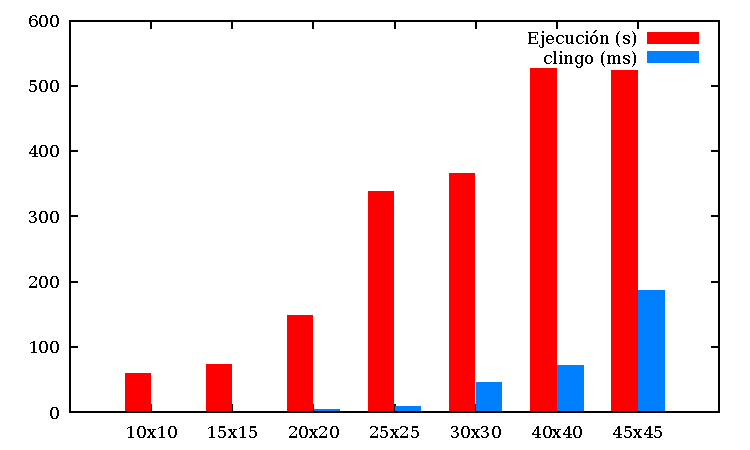
\includegraphics[width=.8\textwidth]{tables/map-size.pdf}
	\caption{Tiempos del \textit{benchmark} con diferentes tamaños de mapa.}\label{fig:mapresult}
\end{figure}

Con esto nos aseguramos de que cada uno de los módulos tengan porciones parecidas para computar. En la Tabla \ref{table:mapresult} podemos ver los resultados de la realización de esta prueba de rendimiento ejecutando 25 ejecuciones cada una de las medidas, en donde se recoge el tiempo total de todas las ejecuciones, el tiempo total que ha usado clingo para obtener una solución y el tiempo medio de una ejecución. Por otra parte en la Figura \ref{fig:mapresult} podemos ver una comparativa entre el tiempo medio entre ejecuciones y el tiempo medido arrojado por clingo. \\

Como se puede observar, el tiempo de ejecución sigue una tendencia casi exponencial, haciendo que a partir de mapas de 45x45 celdas en ningún momento la ejecución tarde menos de 5 minutos. Aún así, hay que destacar un caso concreto, ya que la prueba de un mapa de 35x35 celdas con los valores propuestos se realiza en más de 5 minutos, cosa que tanto en las pruebas anteriores como en las siguientes no ocurre. Esto puede deberse a que el mapa para esta prueba no esté bien repartido para los distintos módulos.  

\section{Porcentajes de tierra y biomas}
\label{sec:pruebatierrabiomas}

Para la primera parte de la prueba se ha usado distintos porcentajes de tierra, usando la cantidad de islas y los parámetros de cantidad y tamaño de los cuadrantes para mapas de 25x25 celdas de la prueba anterior y dejando el resto de variables con valores por defecto (cantidad de biomas al 20\%, tamaño de las cordilleras en 2 casillas, longitud de cordilleras en 3 casillas, 2 jugadores y 2 casillas de distancia mínima entre jugadores). \\

\begin{table}[!h]
	\centering
	\begin{tabular}{ c c c c }
		\bfseries{Porcentaje} & \bfseries{Total}  & \bfseries{clingo} & \bfseries{Ejecución} \\
		\hline
		10\% & 174 s & 565 ms & 6,96 s \\
		15\% & 178 s & 601 ms & 7,12 s \\
		20\% & 178 s & 612 ms & 7,12 s \\
		25\% & 179 s & 599 ms & 7,16 s \\
		30\% & 181 s & 674 ms & 7,24 s \\
		35\% & 178 s & 565 ms & 7,12 s \\
		40\% & 179 s & 634 ms & 7,16 s \\
		45\% & 178 s & 611 ms & 7,12 s \\
		50\% & 181 s & 627 ms & 7,24 s \\
		55\% & 179 s & 644 ms & 7,16 s \\
		60\% & 178 s & 629 ms & 7,12 s \\
		65\% & 179 s & 598 ms & 7,16 s \\
		70\% & 178 s & 582 ms & 7,12 s \\
		75\% & 180 s & 588 ms & 7,20 s \\
		80\% & 180 s & 636 ms & 7,20 s \\
		\hline
	\end{tabular}
	\caption{Resultado del \textit{benchmark} con diferentes porcentajes de tierra.}\label{table:landresult}
\end{table}

\begin{figure}[!h]
	\centering
	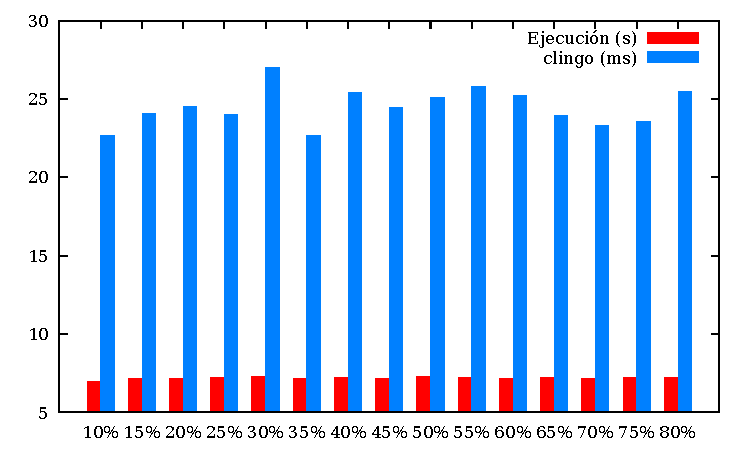
\includegraphics[width=.9\textwidth]{tables/land-size.pdf}
	\caption{Tiempos del \textit{benchmark} con diferentes porcentajes de tierra.}\label{fig:landresult}
\end{figure}

En la Tabla \ref{table:landresult} podemos ver los resultados de la realización de esta prueba de rendimiento ejecutando 25 ejecuciones cada una de las medidas, en donde se recoge el tiempo total de todas las ejecuciones, el tiempo total que ha usado clingo para obtener una solución y el tiempo medio de una ejecución. Por otra parte en la Figura \ref{fig:landresult} podemos ver una comparativa entre el tiempo medio entre ejecuciones y el tiempo medido arrojado por clingo. \\

En el caso de la segunda parte de la prueba se ha usado distintos porcentajes de cantidad de bioma que alcanza una isla, usando los mismos datos que para la prueba anterior. En la Tabla \ref{table:biomaresult} podemos ver los resultados de la realización de esta prueba de rendimiento ejecutando 25 ejecuciones cada una de las medidas, en donde se recoge el tiempo total de todas las ejecuciones, el tiempo total que ha usado clingo para obtener una solución y el tiempo medio de una ejecución. Por otra parte en la Figura \ref{fig:biomaresult} podemos ver una comparativa entre el tiempo medio entre ejecuciones y el tiempo medido arrojado por clingo.

\begin{table}[!h]
	\centering
	\begin{tabular}{ c c c c }
		\bfseries{Porcentaje} & \bfseries{Total}  & \bfseries{clingo} & \bfseries{Ejecución} \\
		\hline
		10\% & 178 s & 635 ms & 7,12 s \\
		15\% & 180 s & 621 ms & 7,20 s \\
		20\% & 179 s & 603 ms & 7,16 s \\
		25\% & 178 s & 636 ms & 7,12 s \\
		30\% & 178 s & 614 ms & 7,12 s \\
		35\% & 179 s & 586 ms & 7,16 s \\
		40\% & 179 s & 612 ms & 7,16 s \\
		45\% & 213 s & 634 ms & 8,52 s \\
		50\% & 215 s & 675 ms & 8,60 s \\
		55\% & 216 s & 758 ms & 8.64 s \\
		60\% & 207 s & 705 ms & 8,28 s \\
		65\% & 192 s & 683 ms & 7,68 s \\
		70\% & 187 s & 688 ms & 7,48 s \\
		75\% & 208 s & 693 ms & 8,32 s \\
		80\% & 204 s & 658 ms & 8,16 s \\
		\hline
	\end{tabular}
	\caption{Resultado del \textit{benchmark} con diferentes porcentajes de tierra.}\label{table:biomaresult}
\end{table}

\begin{figure}[!h]
	\centering
	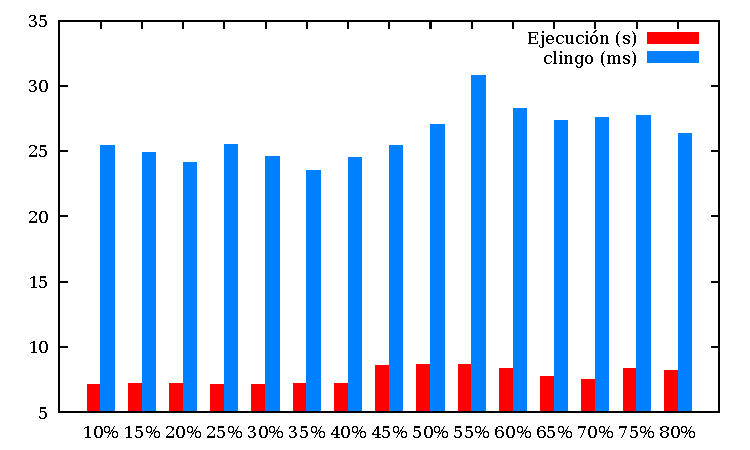
\includegraphics[width=0.9\textwidth]{tables/bioma-size.pdf}
	\caption{Tiempos del \textit{benchmark} con diferentes porcentajes de tierra.}\label{fig:biomaresult}
\end{figure}

Como se puede observar, en estas pruebas no se haya bastante diferencia al modificar uno de los valores, dando resultados muy similares entre si. Es por eso que se ha decidido combinar las dos pruebas en una sola para observar algún cambio efectivo. Esto se recoge en la Sección \ref{sec:pruebafinal}.

\section{Prueba mixta tierra/biomas}
\label{sec:pruebafinal}

En esta última prueba se ha tenido en cuenta los datos de la prueba relatada en la Sección \ref{sec:pruebatierrabiomas}, es decir, usando un mapa de 25x25 dividido en 5 cuadrantes de 5 celdas cada uno, con 4 islas totales y dejando el resto de variables con valores por defecto (tamaño de las cordilleras en 2 casillas, longitud de cordilleras en 3 casillas, 2 jugadores y 2 casillas de distancia mínima entre jugadores).

\begin{table}[!h]
	\centering
	\begin{tabularx}{\textwidth}{c|cccccccccccc}
	 & \multicolumn{2}{c}{10\%} & \multicolumn{2}{c}{15\%} & \multicolumn{2}{c}{20\%} & \multicolumn{2}{c}{25\%} & \multicolumn{2}{c}{30\%} & \multicolumn{2}{c}{35\%} \\
	\hline
	10\% & 42 & 148 & 41 & 167 & 35 & 152 & 88 & 187 & 117 & 189 & 214 & 183 \\
	15\% & 41 & 204 & 37 & 147 & 36 & 127 & 88 & 185 & 133 & 191 & 247 & 182 \\
	20\% & 37 & 165 & 43 & 155 & 37 & 139 & 105 & 188 & 123 & 191 & 224 & 185 \\
	25\% & 29 & 140 & 51 & 171 & 43 & 138 & 92 & 185 & 123 & 190 & 220 & 181 \\
	30\% & 42 & 193 & 43 & 159 & 138 & 131 & 95 & 189 & - & - & - & - \\
	35\% & 41 & 171 & 40 & 175 & 38 & 139 & 90 & 186 & - & - & 241 & 183 \\
	40\% & 43 & 203 & 46 & 188 & 36 & 134 & - & - & - & - & 217 & 183 \\
	45\% & 69 & 203 & 49 & 186 & 36 & 156 & 737 & 192 & - & - & 220 & 184 \\
	50\% & 100 & 179 & - & - & 1064 & 850 & - & - & - & - & - & - \\
	55\% & 55 & 192 & 956 & 170 & - & - & - & - & - & - & - & - \\
	60\% & 164 & 204 & 740 & 178 & - & - & - & - & - & - & - & - \\
	65\% & 97 & 187 & 838 & 132 & - & - & - & - & - & - & - & - \\
	\hline
	\end{tabularx}
	\caption{Resultado del \textit{benchmark} con diferentes porcentajes de tierra (las columnas) y de biomas (las filas). Los tiempos totales son en segundos (la primera celda), y los tiempos de clingo son en milisegundos (la segunda celda)}\label{table:finalresult}
\end{table}

Como se puede observar en los resultado mostrados en la Tabla \ref{table:finalresult}, en donde se han ejecutado 5 iteraciones por cada valor, el módulo de clingo obtiene resultados decentes cuando se establecen valores bajos para el porcentaje de tierra y de biomas, más el tiempo de ejecución se dispara en el momento de poner valores altos. Esto se debe a, como ya se ha comentado a lo largo de la memoria, el paradigma ASP puede llegar a tener en cuenta una gran combinación de datos y producirse una explosión combinatoria de soluciones, retardando en buena medida la procura de una solución.